\section{Bestrahlungsplanung}
\label{sec:Bestrahlungsplanung}

Das PTV ist in den CT-Daten bereits eingezeichnet und als nächstes wurde die Kontur der Hüfte als Body-Struktur eingezeichnet.
Andere Gegenstände, wie z.B. Lagerungshilfe oder Patientenliege, werden auch als Struktur eingezeichnet, weil sich diese auch in dem Strahlengang befinden.
Das Ziel der Bestrahlungsplanung ist, dass das Planungszielvolumen durch die $\SI{95}{\percent}$ Isodosenlinie umschlossen wird.
Für die Bestrahlungsplanung wurden zwei Felder mit einer Gewichtung von jeweils $\SI{50}{\percent}$ erzeugt.
Die beiden Felder sind gleich groß und haben eine Größe
von  $\SI{14}{\centi\meter}$ x $\SI{11.5}{\centi\meter}$. Beim ersten Feld beträgt die Gantry-Rotation $0^\circ$ und bei dem zweiten Feld $180^\circ$.
Der Bestrahlungsplan wird auf "$\SI{100}{\percent}$ target mean" normiert.
Für die Schonung des umliegenden Gewebes werden MLCs verwendet, die an das PTV angepasst werden.
Die Einstellung der MLCs ist in der Abbildung \ref{abb:MLC} zu sehen.


\begin{figure}[H]
  \centering
  \begin{subfigure}{\textwidth}
    \centering
    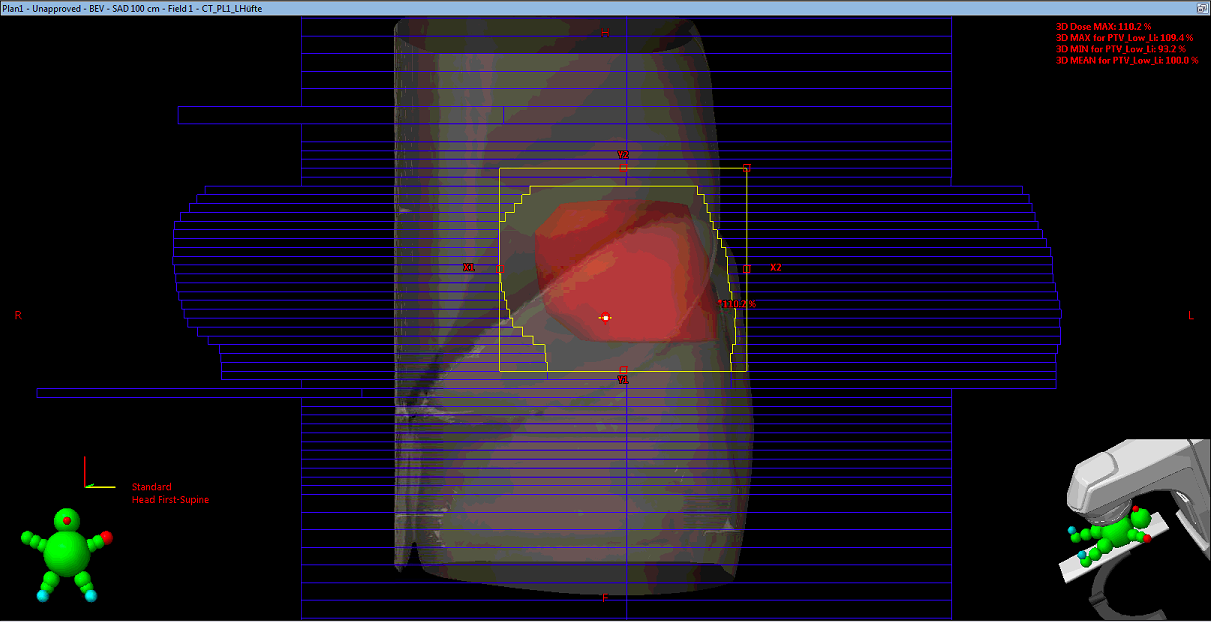
\includegraphics[height = 5cm]{Bilder/MLC_Hüfte1.png}
    \caption{}
  \end{subfigure}
  \begin{subfigure}{\textwidth}
    \centering
    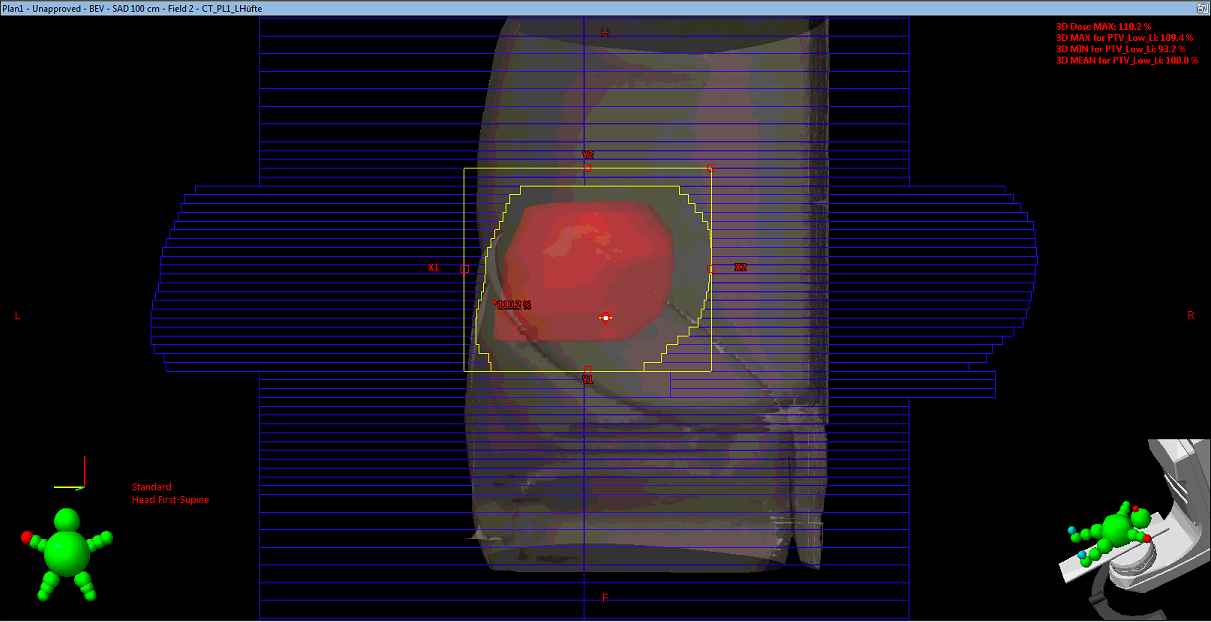
\includegraphics[height=5cm]{Bilder/MLC_Hüfte2.png}
    \caption{}
  \end{subfigure}
  \caption{Darstellung der Lamellenpositionen der beiden Felder. Bei a) die Positionen bei dem Feld bei $0°$ und bei b) die Positionen bei dem Feld bei $180°$.}
  \label{abb:MLC}
\end{figure}
